\subsection{Main Comparison Across Load Scenarios}

\begin{figure}[h]
    \centering
    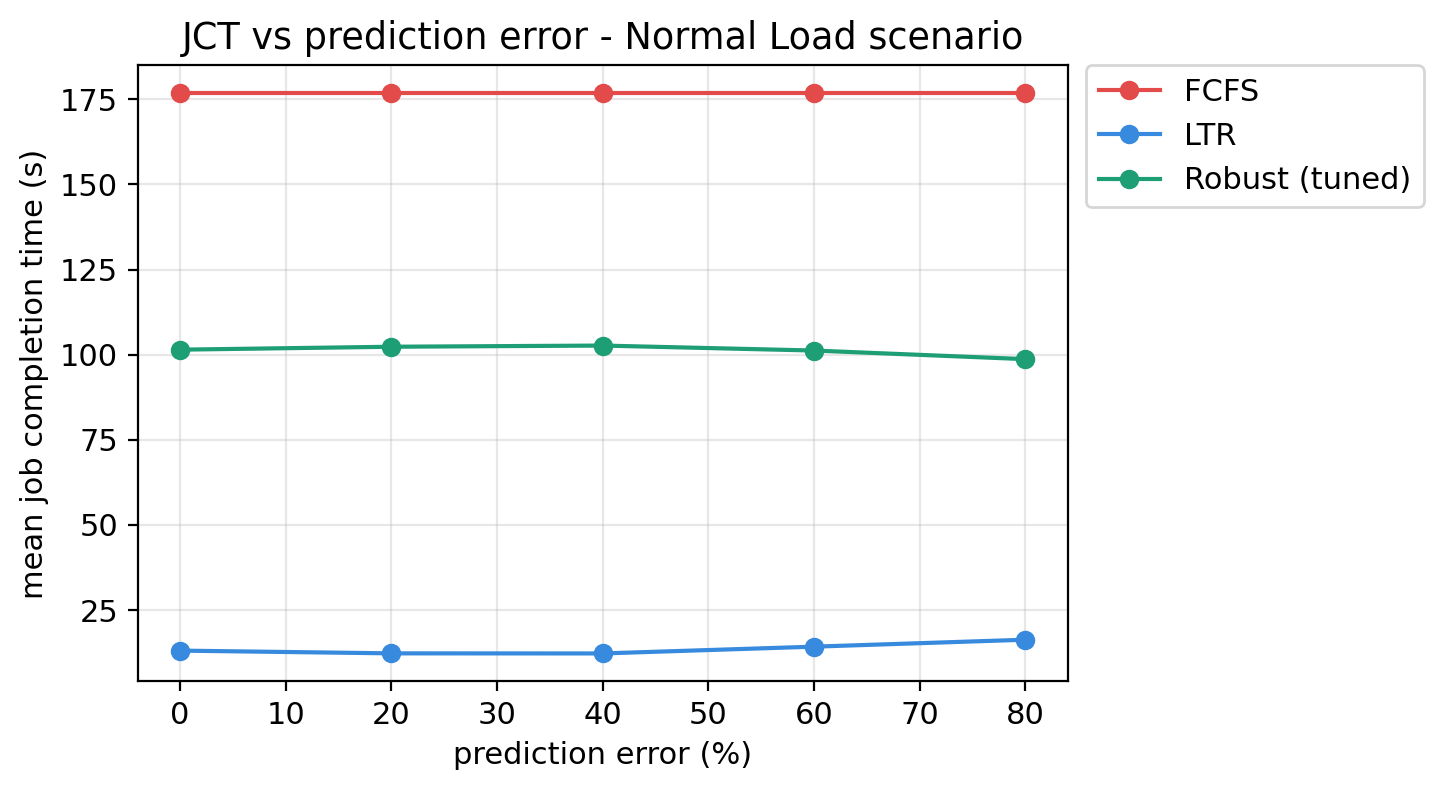
\includegraphics[width=0.92\columnwidth]{figures/fig1_jct_vs_error.png}
    \caption{Mean JCT versus prediction error.}
    \label{fig:jct_error}
\end{figure}

\begin{figure}[h]
    \centering
    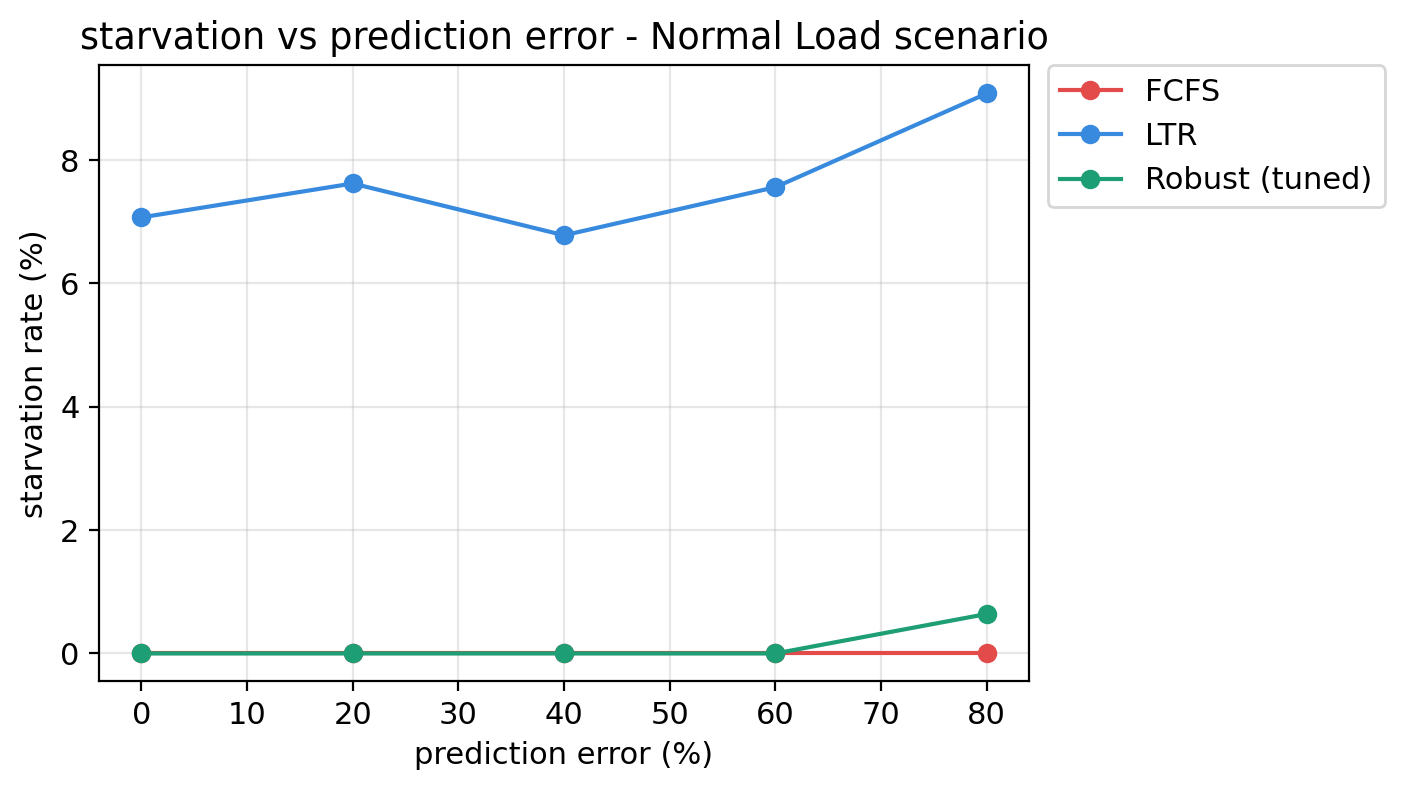
\includegraphics[width=0.92\columnwidth]{figures/fig2_starvation_vs_error.png}
    \caption{Starvation rate versus prediction error.}
    \label{fig:starvation_error}
\end{figure}

Figures~\ref{fig:jct_error} and~\ref{fig:starvation_error} compare the three scheduling strategies under the Normal load scenario across prediction error levels ranging from 0\% to 80\%. LTR consistently achieves the lowest mean job completion time (JCT), while FCFS produces the highest JCT under all evaluated conditions. The proposed Robust scheduler remains between these two baselines, maintaining a substantially lower JCT than FCFS while avoiding the extremely aggressive scheduling behavior of LTR.

Although LTR reports the lowest average JCT, this should not be interpreted as the best overall scheduling performance. Across all evaluated prediction error levels, LTR experiences a starvation rate between 6.78\% and 9.08\%, meaning it completes only about 910--930 of the 1,000 requests. In contrast, the proposed Robust scheduler maintains a starvation rate between 0\% and 0.64\%, completing approximately 994--1,000 requests. Its average JCT is therefore measured over a substantially larger and more representative set of completed requests, including difficult requests that LTR tends to abandon, which explains why the Robust scheduler reports a higher average JCT while providing fairer and more reliable scheduling performance under prediction uncertainty.

\subsection{Parameter Sensitivity and Grid Refinement}

\begin{figure}[h]
    \centering
    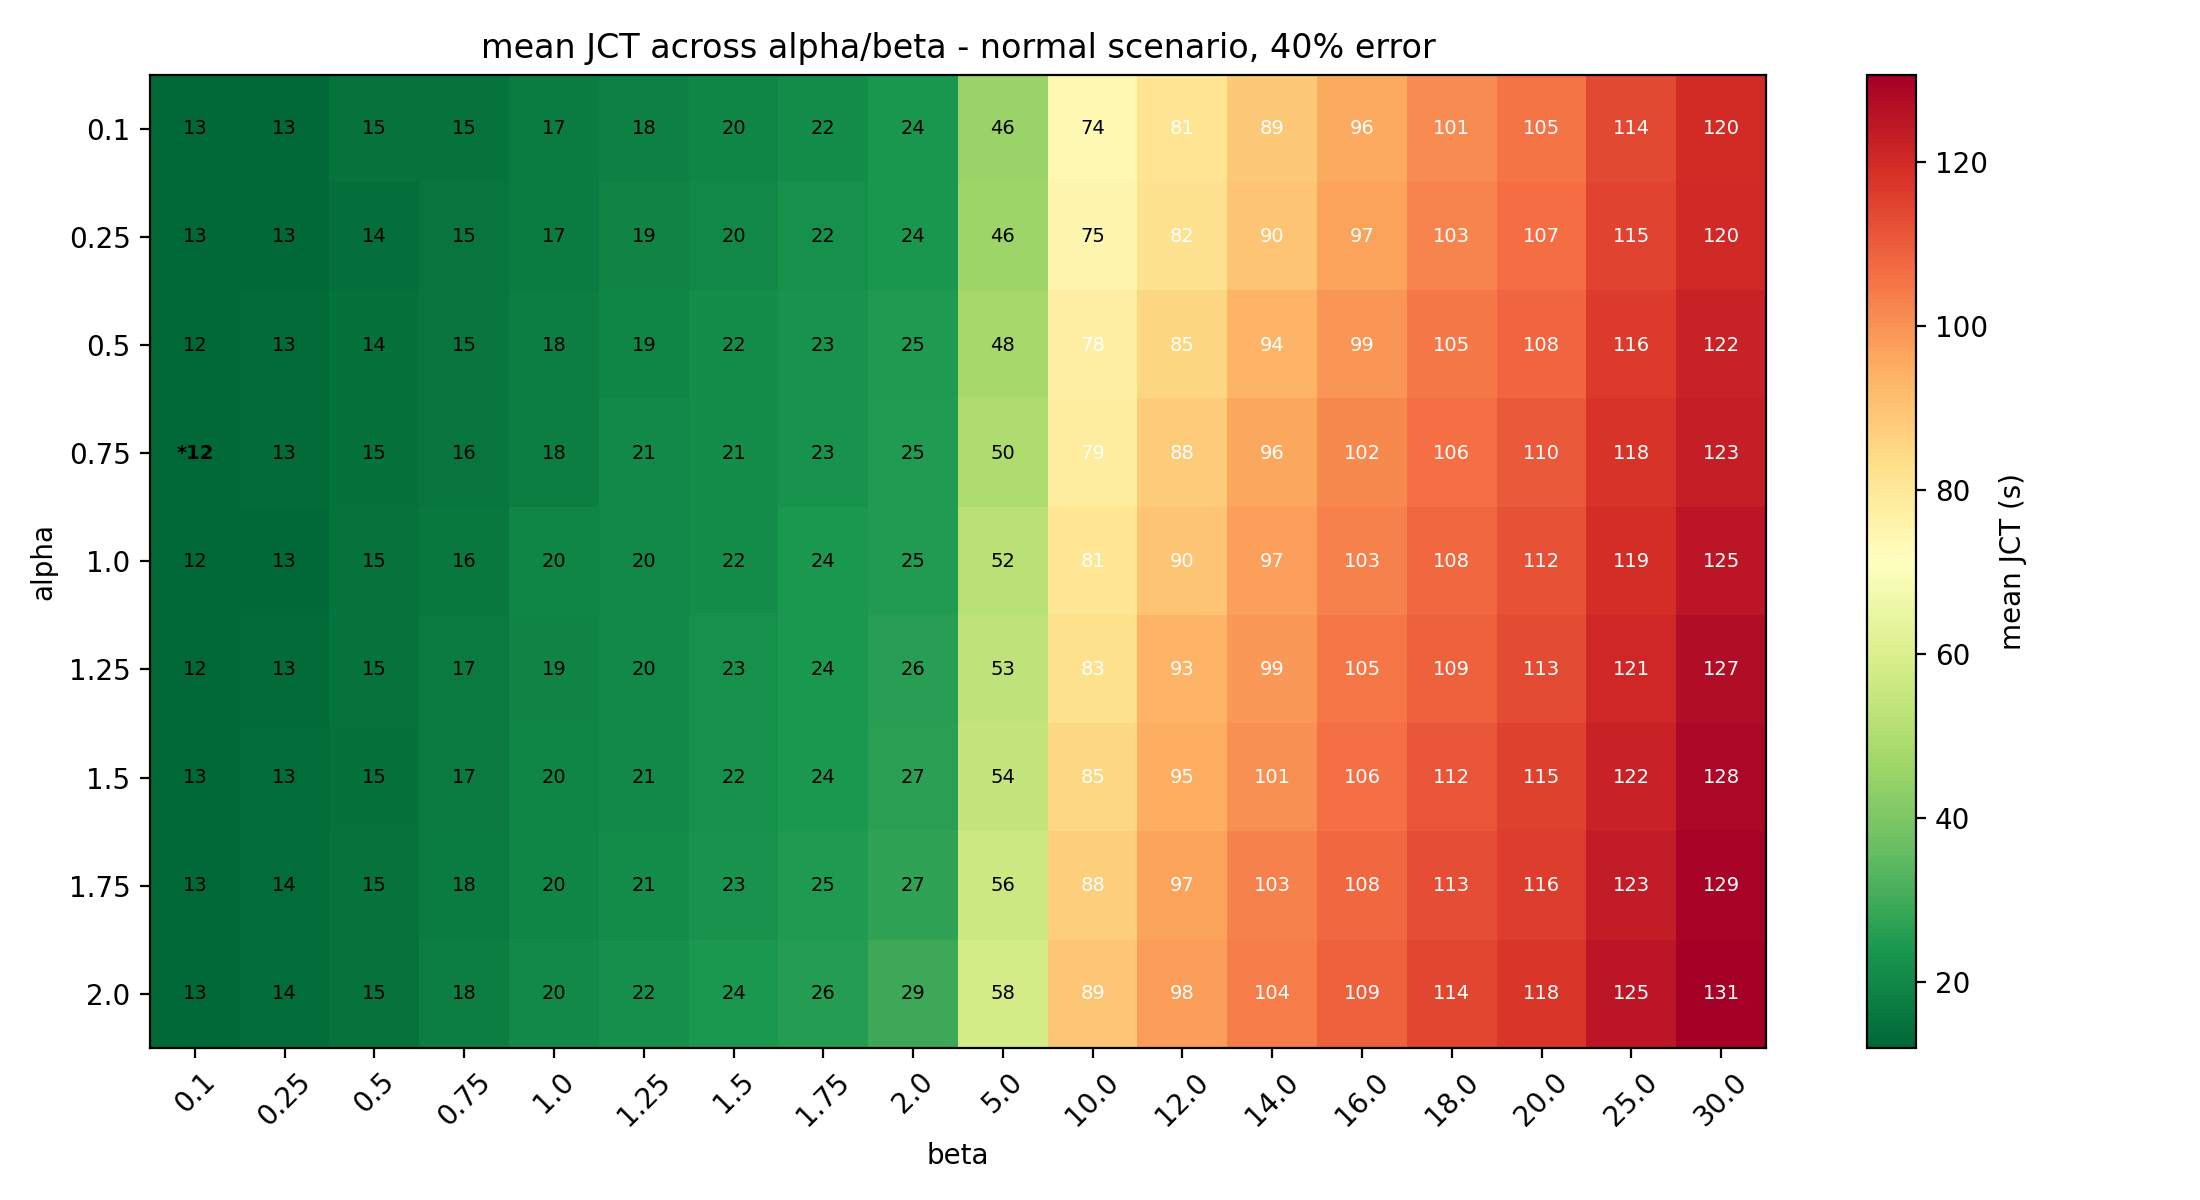
\includegraphics[width=\columnwidth]{figures/fig3_heatmap.png}
    \caption{Mean JCT across the alpha/beta grid.}
    \label{fig:heatmap}
\end{figure}

Fig.~\ref{fig:heatmap} shows the mean completion time for every alpha and beta pair we tested, for the Normal scenario at 40\% prediction error. One thing stood out once we looked closely: starvation does not fall in a straight line as beta goes up, it actually gets worse for a while before it starts getting better. Our first grid jumped straight from beta equal to 10 to beta equal to 20, so this was missed entirely at first, and the grid search picked beta equal to 20 as the answer simply because it was the next point tested, not because it was the cheapest point that actually worked. Filling in the points in between revealed the real turning point closer to beta equal to 17 or 18, and using that value instead of 20 lowered the average completion time by roughly 5 to 7 percent across scenarios, without giving up the fairness constraint required.

\begin{figure}[h]
    \centering
    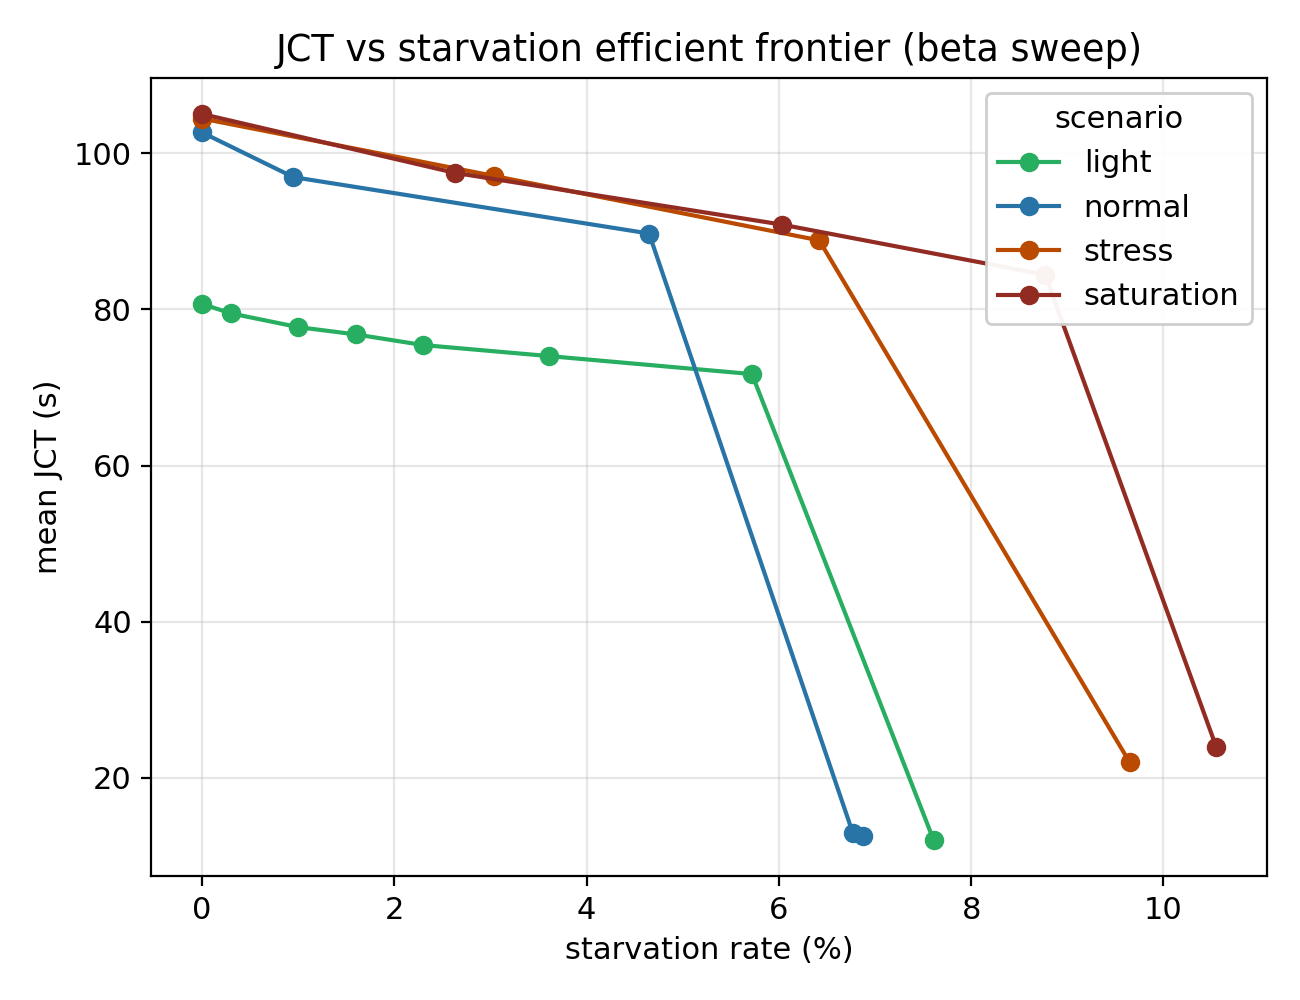
\includegraphics[width=\columnwidth]{figures/fig5_pareto.png}
    \caption{JCT-starvation efficient frontier.}
    \label{fig:pareto}
\end{figure}

Fig.~\ref{fig:pareto} only keeps the settings where nothing else in the tested range beats them on both completion time and starvation at once. This is what makes the final chosen setting for each scenario defendable: it is not a point that happened to look good in isolation, it is a point that nothing else on the same list dominates.

\subsection{Ablation Study}
\begin{figure}[h]
    \centering
    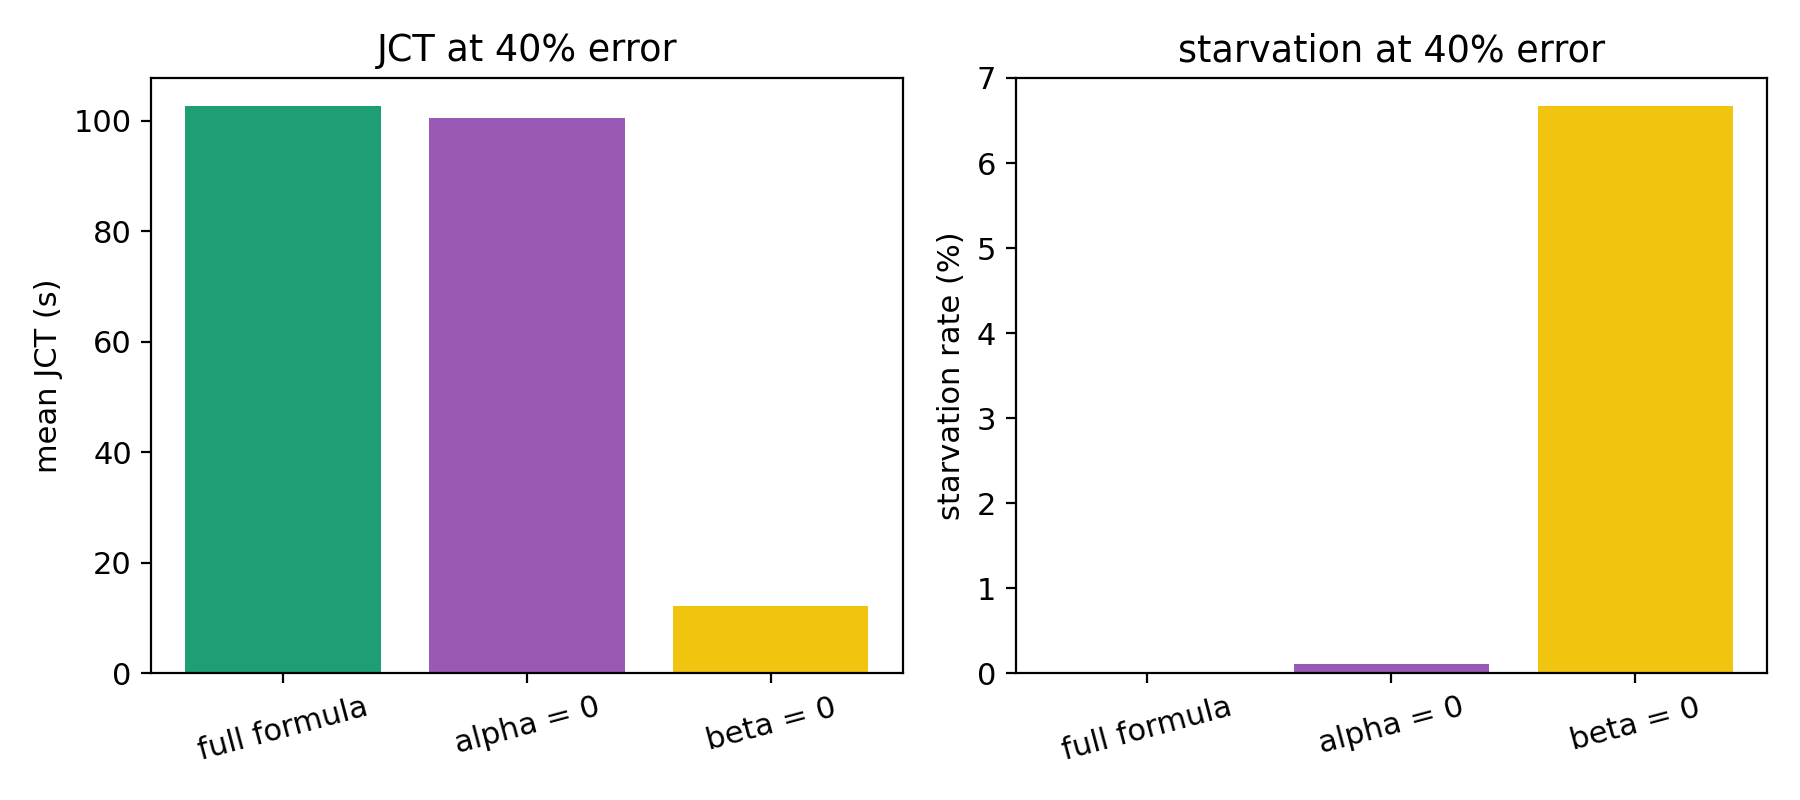
\includegraphics[width=\columnwidth]{figures/fig4_ablation.png}
    \caption{Ablation of the alpha and beta terms.}
    \label{fig:ablation}
\end{figure}
Fig.~\ref{fig:ablation} shows the ablation results in the Normal scenario at a 40\% prediction-error rate. The baseline gives a mean JCT of 102.66~s and a starvation rate of 0\%. Setting $\alpha = 0$ lowers mean JCT slightly to 100.43~s, and raises starvation only marginally, to 0.11\%. Setting $\beta = 0$ has a much larger effect: mean JCT falls to 12.15~s, starvation rises to 6.67\%, and 8.5\% of requests time out, close to LTR's own mean JCT of 12.19~s, starvation rate of 6.78\%, and timeout rate of 8.5\% under the same conditions.

The low JCT at $\beta = 0$ does not represent better overall performance, since JCT is calculated only for completed requests. Without aging, the scheduler favors short requests and more long requests time out, so the mean reflects an easier set of jobs. The aging term raises a request's priority as waiting time increases and is the main protection against starvation, using the same basic idea as Highest Response Ratio Next (HRRN) \cite{hansen1973os}. At 40\% error, removing alpha barely changes starvation at all, which shows beta is carrying nearly all of the fairness protection on its own at this operating point, while alpha's own contribution here is small.

\subsection{Fairness Across Schedulers}
\begin{figure}[h]
    \centering
    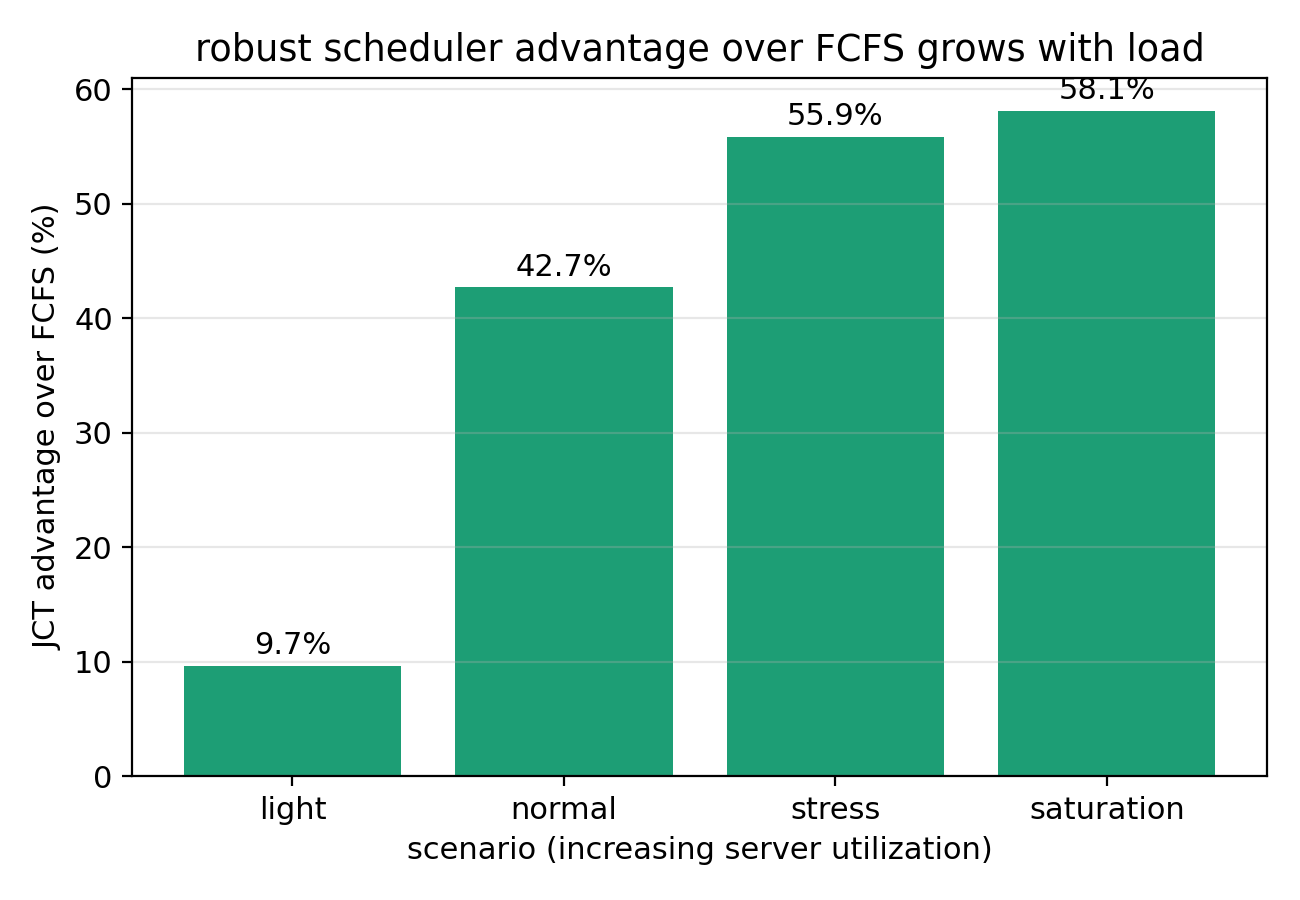
\includegraphics[width=\columnwidth]{figures/fig6_advantage_vs_fcfs.png}
    \caption{JCT advantage over FCFS by scenario.}
    \label{fig:advantage}
\end{figure}

\begin{figure}[h]
    \centering
    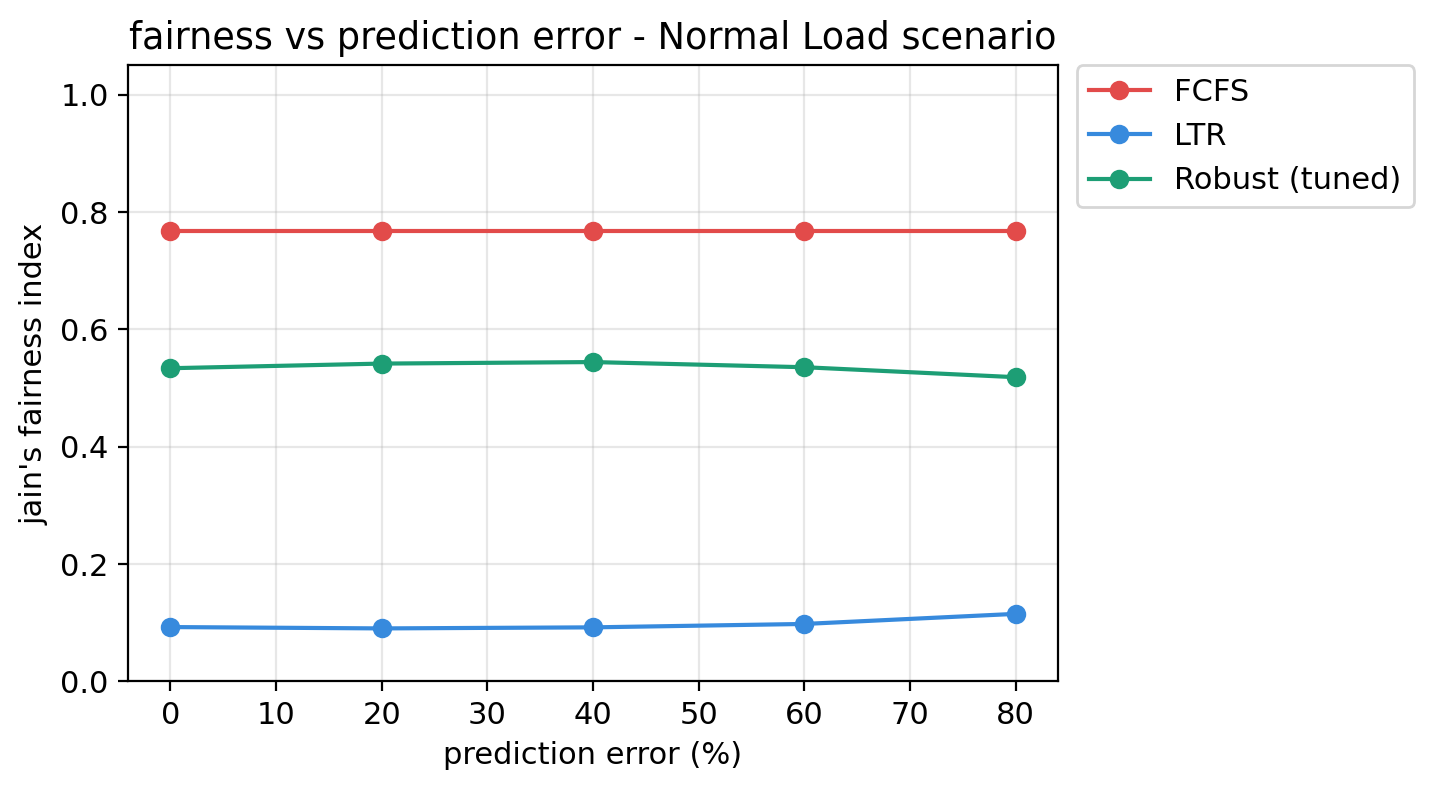
\includegraphics[width=\columnwidth]{figures/fig7_jains_fairness.png}
    \caption{Jain's fairness index versus prediction error.}
    \label{fig:jains}
\end{figure}
Fig.~\ref{fig:advantage} shows the reduction in mean JCT relative to FCFS, averaged over all five prediction-error levels: 9.7\% under Light load, 42.7\% under Normal load, 55.9\% under Stress load, and 58.1\% under Saturation load. Under light load, queues are relatively short, giving FCFS fewer opportunities to place a large request ahead of many short ones. As system utilization increases, longer queues make head-of-line blocking more severe, and by considering both predicted request size and waiting time, the proposed scheduler reduces this effect.

Fig.~\ref{fig:jains} compares Jain's fairness index under the Normal workload. FCFS achieves the highest fairness index, 0.7675, but also the highest mean JCT at 176.75~s, because Jain's index measures how evenly completion times are distributed among completed requests rather than whether those completion times are low. LTR produces much lower fairness values, ranging from 0.09 to 0.12, since it strongly favors shorter predicted requests. The proposed scheduler falls between the two extremes, with fairness values between 0.52 and 0.54 while keeping starvation between 0\% and 0.64\%, compared with 6.78\% to 9.08\% for LTR.

\subsection{Robustness to Out-of-Distribution Predictions}
The out-of-distribution (OOD) noise model differs from the bounded symmetric prediction errors used in the previous experiments. Instead of introducing small errors to every request, only a fraction of requests receive prediction values that are largely unrelated to their true execution cost, representing previously unseen request patterns and providing a more challenging evaluation of scheduler robustness \cite{kumar2024latency}.


\begin{figure}[h]
    \centering
    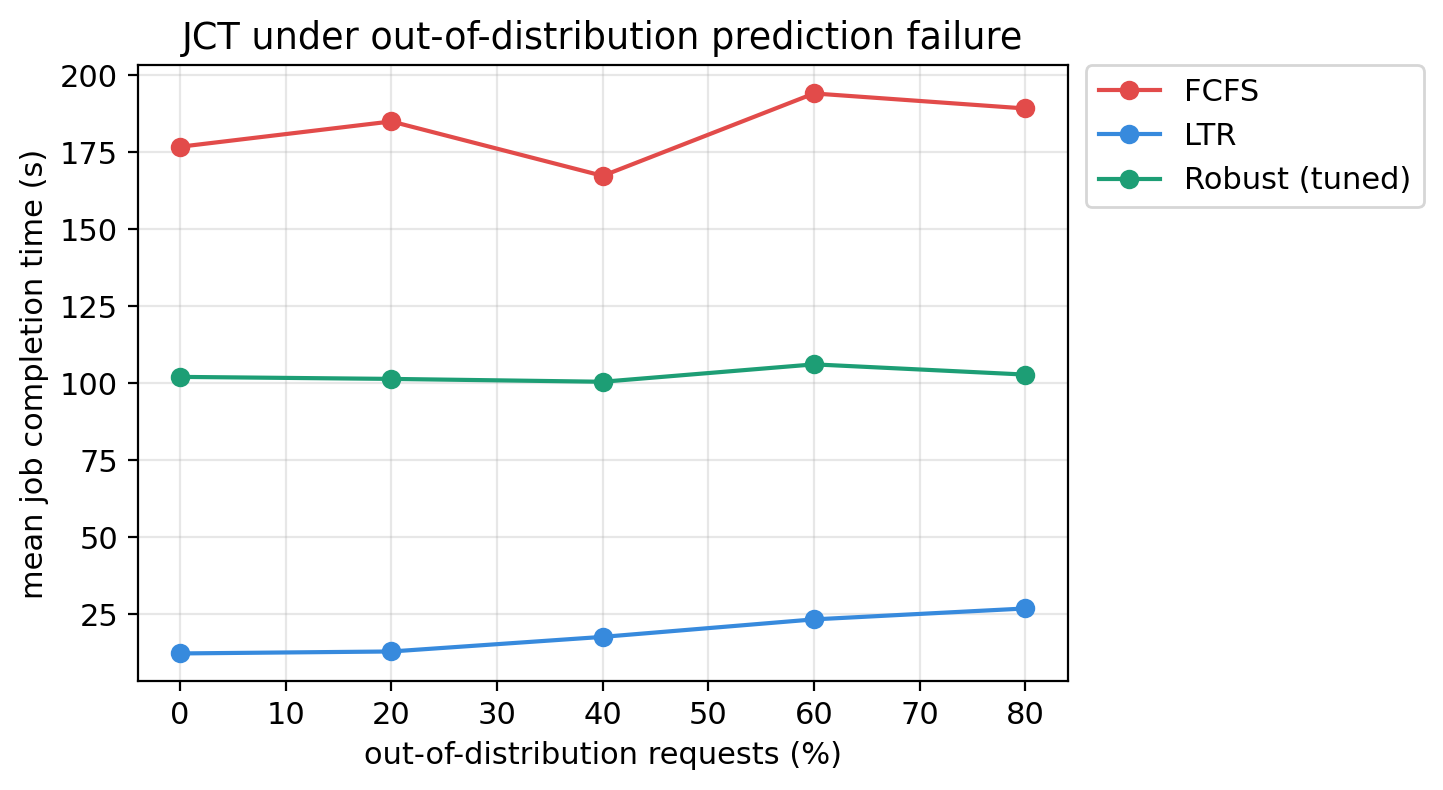
\includegraphics[width=0.92\columnwidth]{figures/fig8_ood_jct.png}
    \caption{Mean JCT under out-of-distribution noise.}
    \label{fig:ood_jct}
\end{figure}

\begin{figure}[h]
    \centering
    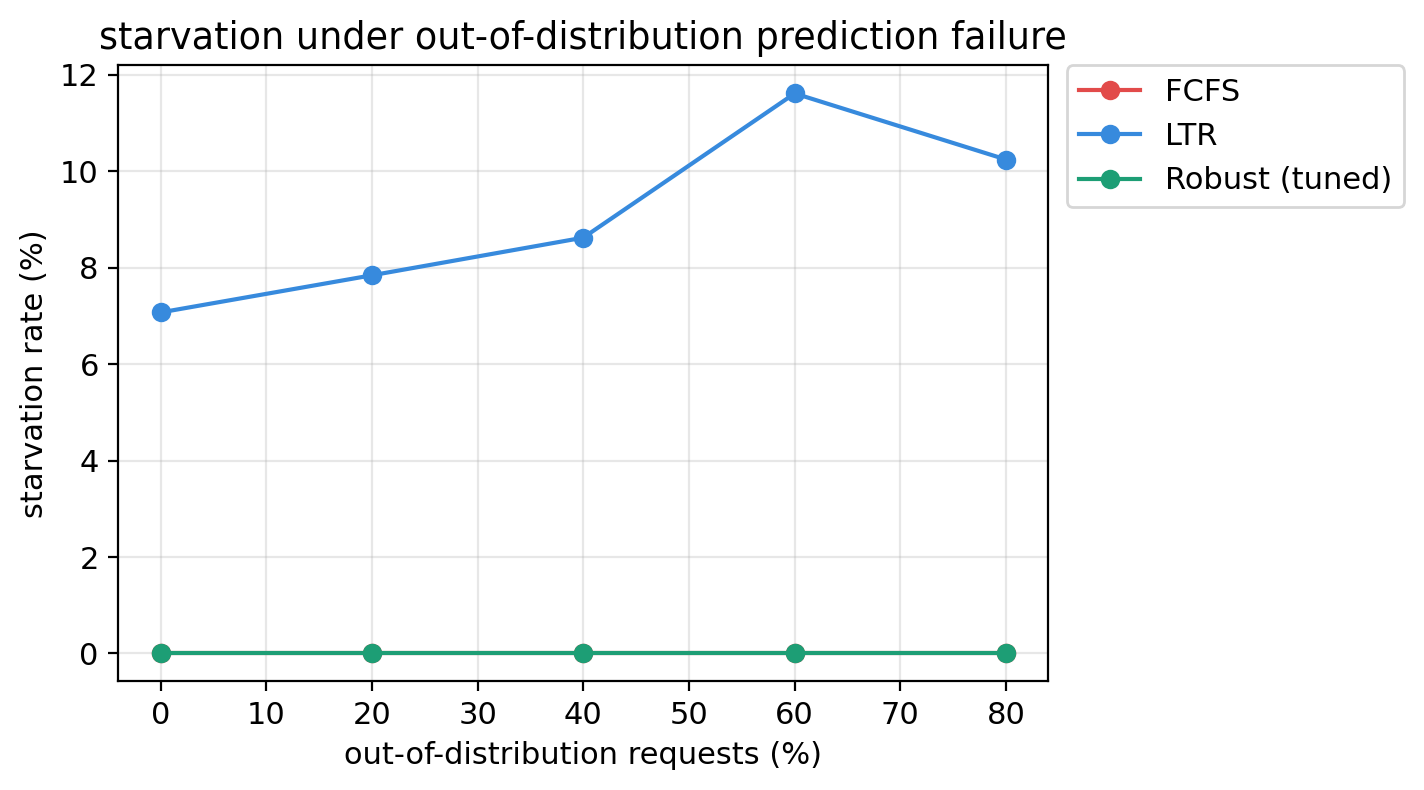
\includegraphics[width=0.92\columnwidth]{figures/fig9_ood_starvation.png}
    \caption{Starvation under out-of-distribution noise.}
    \label{fig:ood_starvation}
\end{figure}


As shown in Figures~\ref{fig:ood_jct} and~\ref{fig:ood_starvation}, the proposed Robust scheduler remains stable across all out-of-distribution levels: mean JCT changes only slightly, and the starvation rate stays close to zero. LTR, in contrast, becomes increasingly sensitive to prediction failures, with its starvation rate rising from approximately 7\% to over 10\% and its mean JCT increasing as more requests become out-of-distribution. These results suggest that incorporating prediction uncertainty into scheduling decisions helps maintain reliable performance even when prediction models encounter previously unseen request patterns \cite{kumar2024latency, fu2024ltr}.
